\subsection{vLLM Performance Dashboard}
{{\footnotesize
\noindent A live visual dashboard for vLLM showcasing throughput, latency, and other inference metrics across models and hardware configurations.


\begin{description}[labelwidth=4cm, labelsep=1em, leftmargin=4cm, itemsep=0.1em, parsep=0em]
  \item[date:] 2022-06-22
  \item[version:] v1.0
  \item[last\_updated:] 2025-01
  \item[expired:] unknown
  \item[valid:] yes
  \item[valid\_date:] 2022-06-22
  \item[url:] \href{https://simon-mo-workspace.observablehq.cloud/vllm-dashboard-v0/}{https://simon-mo-workspace.observablehq.cloud/vllm-dashboard-v0/}
  \item[doi:] unknown
  \item[domain:] LLM; HPC/inference
  \item[focus:] Interactive dashboard showing inference performance of vLLM
  \item[keywords:]
    - Dashboard
    - Throughput visualization
    - Latency analysis
    - Metric tracking
  \item[licensing:] unknown
  \item[task\_types:]
    - Performance visualization
  \item[ai\_capability\_measured:]
    - Throughput
    - latency
    - hardware utilization
  \item[metrics:]
    - Tokens/sec
    - TTFT
    - Memory usage
  \item[models:]
    - LLaMA-2
    - Mistral
    - Qwen
  \item[ml\_motif:]
    - HPC/inference
  \item[type:] Framework
  \item[ml\_task:]
    - Visualization
  \item[solutions:] 0
  \item[notes:] Built using ObservableHQ; integrates live data from vLLM benchmarks.
The URL requires a login to access the content.

  \item[contact.name:] Simon Mo
  \item[contact.email:] unknown
  \item[results.links.name:] ChatGPT LLM
  \item[fair.reproducible:] Yes
  \item[fair.benchmark\_ready:] Yes
  \item[id:] vllm\_performance\_dashboard
  \item[Citations:] \cite{mo2024vllm_dashboard}
\end{description}

{\bf Ratings:} ~ \\

\begin{tabular}{p{0.15\textwidth} p{0.07\textwidth} p{0.7\textwidth}}
\hline
Rating & Value & Reason \\
\hline
dataset & 2 & No datasets are bundled; the dashboard visualizes metrics derived from model
inference logs or external endpoints, not a formal dataset.
 \\
documentation & 4 & Public dashboard with instructions and tooltips; documentation is clear, though access
is restricted (login required) and backend setup is opaque to users.
 \\
metrics & 4 & Tracks tokens/sec, TTFT, memory usage, and platform comparisons. Metrics are clear
but focused on visualization rather than statistical robustness.
 \\
reference\_solution & 3 & Dashboards include reproducible views of benchmarked models, but do not ship
with runnable model code. Relies on external serving infrastructure.
 \\
software & 4 & Interactive dashboard built with ObservableHQ and linked to vLLM benchmarks.
Source code is not fully open, but backend integration with vLLM is well-maintained.
 \\
specification & 4 & While primarily a visualization tool, it includes benchmark configurations,
metric definitions, and supports comparison across models and hardware.
 \\
\hline
\end{tabular}

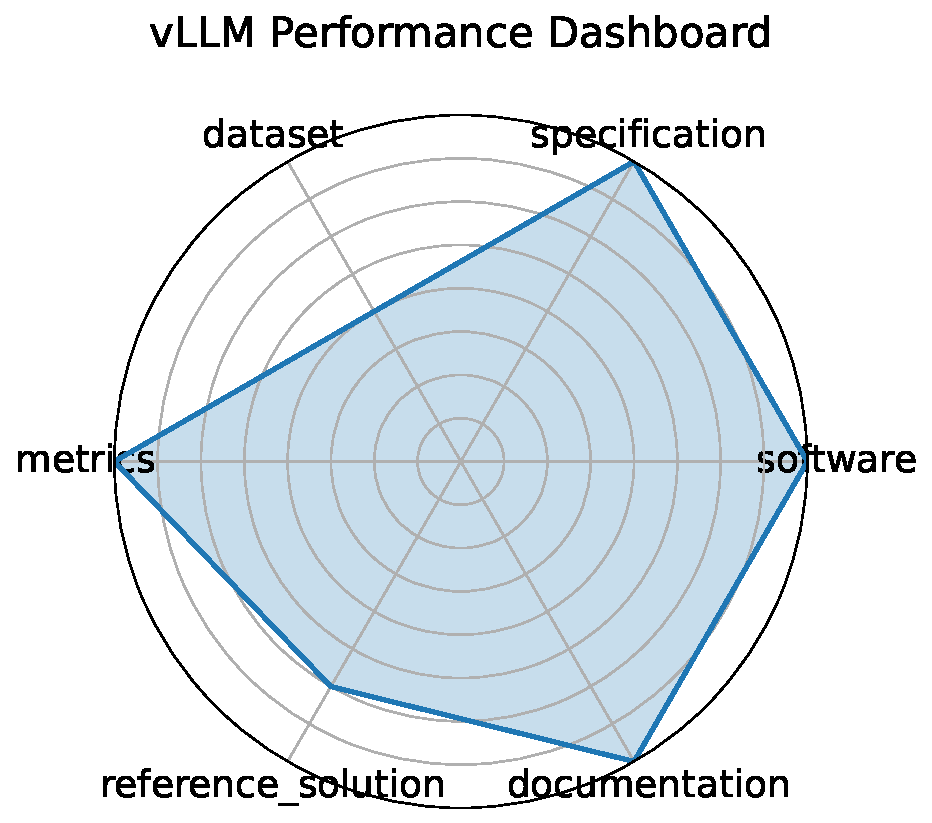
\includegraphics[width=0.2\textwidth]{vllm_performance_dashboard_radar.pdf}
}}
\clearpage